\chapter{Trabalhos Relacionados}\label{chap:revisao}

\section{Considerações Iniciais}

Os trabalhos que mais se relacionam ao o aqui proposto são
aqueles que transformam os conjuntos de dados em busca de
uma melhor representação do problema em estudo. Esses
trabalhos se dividem basicamente em dois grupos: métodos de
redução de dimensionalidade e métodos de transformação
interativa do espaço de atributos. Deste modo, a seguir
apresenta-se uma discussão sobre os métodos da
extensa literatura em redução de dimensionalidade, com um
enfoque especial para métodos interativos. Apresenta-se
também um levantamento sobre pesquisas em transformação
interativa do espaço de atributos, um tema que não conta com uma
literatura tão vasta quanto à dos métodos de redução, mas
que tem ganhado popularidade nos últimos anos.

\section{Redução de Dimensionalidade}

O problema de se a reduzir a dimensionalidade de conjuntos
de dados pode ser descrito da seguinte forma: dado um
conjunto de dados representado por uma matriz $\textbf{X}$
composta por $n$ vetores $\textbf{x}_i~(i \in
\{1,2,...,n\})$ $m-$dimensionais, deseja-se encontrar uma
transformação $t: \textbf{X} \rightarrow \textbf{Y}$, em que 
$\textbf{Y}$ trata-se de uma matriz composta por $n$ vetores
$\textbf{y}_i~(i \in \{1,2,...n\}$ de dimensionalidade $p$
($p < m$).  Normalmente $p \ll m$ e, idealmente, $p$
equivale à dimensionalidade intrínseca dos dados~\footnote{A
dimensionalidade intrínseca dos dados é o conjunto mínimo de
variáveis necessárias para descrever as propriedades dos
dados~\cite{Fukunaga1990}.}, fazendo com que $t$ mantenha em
$\textbf{Y}$ o máximo das propriedades de $\textbf{X}$
quanto for possível. 

Dentre os propósitos da redução de dimensionalidade, os
principais são a melhoria na eficiência dos métodos que
operam sobre os dados e a redução do custo computacional
desses métodos. \cite{Konig2000}, por exemplo, apresenta
melhorias na precisão de sistemas de classificação e no
desempenho de sistemas de reconhecimento automático ao
preceder os procedimentos com o processo de redução de
dimensionalidade. Até mesmo outros benefícios não tão
diretos podem ser alcançados por meio do uso de técnicas de
redução. Trata-se do caso do mesmo trabalho apresentado por
\citeauthor{Konig2000}, onde métodos de redução de
dimensionalidade são utilizados para reduzir a complexidade
de projetos de circuitos integrados, resultando em uma
redução na área e no consumo de energia dos circuitos. Uma
terceira utilidade para os métodos de redução de
dimensionalidade é viabilizar a construção de representações
visuais de dados multidimensionais~\footnote{No contexto de
visualização computacional, conjuntos de dados
multidimensionais são aqueles com mais do que três
atributos.}, permitindo que sejam mapeados em um espaço
bidimensional (tela computador).  Representações visuais dos
dados são cruciais para a análise exploratória de dados,
principalmente para investigações iniciais dos dados, onde
ainda não se conhece as propriedades dos
dados~\cite{Kaski2011}. 

A literatura em redução de dimensionalidade é extensa e os
métodos desenvolvidos apresentam grande diversidade em
relação a aspectos matemáticos e computacionais. Buscando
uma melhor organização, esta seção foi dividida em duas
subseções. A primeira busca descrever sucintamente os
métodos automáticos e apresentar suas limitações,
principalmente evidenciar que a falta da participação do
usuário no processo faz com que muitas vezes os resultados
obtidos não sejam facilmente compreendidos. A segunda
subseção apresenta os métodos que permitem que o usuário
participe do processo de redução de dimensionalidade por
meio da interação com representações visuais. Ao longo da
segunda subseção discute-se que apesar dos métodos
interativos se mostrarem como uma interessante alternativa
aos métodos automáticos,
os mecanismos de interação propostos ainda apresentam
limitações. 

\subsection{Métodos Automáticos}

A redução de dimensionalidade automática pode ser realizada
seguindo duas abordagens. A primeira transforma os atributos
de entrada em um novo conjunto de dimensões que busca
conservar certas propriedades ou relacionamentos do conjunto
original. Por extrair um novo conjunto de atributos a partir
dos dados originais, esta abordagem recebe o nome de
extração de características (\emph{feature extraction}). Já
a segunda abordagem busca selecionar quais dos atributos do
conjunto de dados são realmente relevantes para a análise
segundo algum critério. Como os dados não são modificados,
esta segunda abordagem é chamada de seleção de
características (\emph{feature selection}).

\subsubsection{Extração de Características}

Como apresentado por~\cite{Maaten2009}, existe uma grande
variedade de métodos de extração de características. Não é
intuito desta subseção detalhar cada uma dessas técnicas e
levantar suas limitações particulares, mas sim ilustrar a
limitação que todas apresentam em comum, isto é, retornar
resultados pouco intuitivos para o usuário e impedi-lo de
interagir com os dados. Para este fim, o método de análise
de componentes principais (PCA)~\cite{Joll2002} será
utilizado.

PCA foi um dos primeiros métodos desenvolvidos para a
redução de dimensionalidade~\cite{Pearson1901} e ainda hoje
é um dos mais utilizados. A construção do espaço reduzido se
baseia em criar combinações lineares entre os atributos de
modo que o novo espaço mantenha o máximo da variância nos
dados. Quando existem relações não lineares entre os
atributos, PCA não é capaz de capturá-las. Em situações como
esta, métodos não lineares como  \textit{Multimensional
Scaling} (MDS)~\cite{Cox2002} e \textit{Self Organizing
Maps} (SOM)\cite{Kohonen1990} podem ser utilizados. No
entanto, foi mostrado por \cite{Maaten2009} que em alguns
casos ainda não é claro se os métodos não lineares são
realmente melhores que PCA.

\begin{table}[htbp]
    \caption[Resultado de PCA]{Resultado obtido pela técnica
        PCA para os dados da Tabela~\ref{tab:at}. As novas
        dimensões construídas, ou componentes, são
        combinações lineares das dimensões originais, onde
        cada uma busca capturar características distintas
        das outras. Os componentes são gerados em uma ordem
        decrescente de importância, de modo que o primeiro
        captura mais informação dos dados que o segundo e
        assim por diante. Não existe correspondência entre
        os valores das dimensões construídas e das
        originais, como por exemplo, entre o componente 2 e
        a variável clima do conjunto original.}
    \begin{center}
        \begin{tabular}{|l|c|c|c|c|c|c|}
            \hline
            & \multicolumn{1}{l|}{\textbf{\textit{Comp.1}}}
            & \multicolumn{1}{l|}{\textbf{\textit{Comp.2}}}
            & \multicolumn{1}{l|}{\textbf{\textit{Comp.3}}}
            & \multicolumn{1}{l|}{\textbf{\textit{Comp.4}}}
            & \multicolumn{1}{l|}{\textbf{\textit{Comp.5}}}
            & \multicolumn{1}{l|}{\textbf{\textit{Comp.6}}}
            \\ \hline
            \textbf{Itália} & 0.0796 & -4.7684 & 0.0922 & 0.3013 & 0.3266 & 0.2819 \\ \hline
            \textbf{Espanha} & 0.4513 & -5.7962 & 1.2968 & 0.3819 & 0.9095 & 0.1914 \\ \hline
            \textbf{Croácia} & -1.7908 & -0.8416 & 0.0145 & -1.5911 & 0.1811 & -0.4065 \\ \hline
            \textbf{Brasil} & 3.448 & -0.9062 & 0.2499 & 0.2469 & -0.6788 & -1.0215 \\ \hline
            \textbf{Rússia} & -4.5417 & 4.3595 & -0.0156 & 1.76 & 0.4539 & -0.1299 \\ \hline
            \textbf{Alemanha} & -8.3095 & 0.5446 & 1.9864 & -0.3819 & -0.8144 & 0.0869 \\ \hline
            \textbf{Turquia} & 4.5991 & -2.2306 & -0.3223 & 0.1513 & -0.6417 & 0.2367 \\ \hline
            \textbf{Marrocos} & 5.1923 & -0.0863 & -0.4045 & 0.2746 & -0.5028 & 0.3295 \\ \hline
            \textbf{Peru} & 0.913 & 0.6241 & -0.4731 & 0.4676 & 0.018 & -0.6031 \\ \hline
            \textbf{Nigéria} & 2.5911 & 4.8643 & 0.1585 & -0.6316 & 0.2394 & 0.1379 \\ \hline
            \textbf{França} & -6.6956 & -2.0063 & -2.7319 & -0.2799 & -0.0306 & 0.1222 \\ \hline
            \textbf{México} & 2.7158 & 3.3806 & 0.0858 & -0.6728 & 1.1078 & -0.0102 \\ \hline
        \end{tabular}
    \end{center}
    \label{tab:at-pcs}
\end{table}

Independentemente de quais técnicas se sobressaem sobre as
outras, uma limitação que todas compartilham é a dificuldade
em se compreender o resultado obtido, isto é, o espaço
dimensional gerado tem pouco significado para o usuário. Por
exemplo, para os dados apresentados na Tabela~\ref{tab:at} o
resultado obtido pelo método PCA é o apresentado na
Tabela~\ref{tab:at-pcs}. Observa-se que não existe
correspondência entre os valores das dimensões construídas e
das originais, assim, com base somente neste resultado, o
usuário não é capaz de compreender quais características do
seus dados foram responsáveis por aquele resultado.

Ao utilizar PCA, a redução de dimensionalidade em si ocorre
ao  manter os $k$ primeiros componentes gerados pelo método.
Em tarefas de visualização, por exemplo, é comum escolher
$k=2$ para manter somente os dois primeiros componentes e
então criar uma representação bidimensional dos elementos.
Uma outra possibilidade, menos arbitrária, para definir $k$
é analisar a parcela da variância dos dados que cada
componente captura. Como pode ser observado no gráfico da
Figura~\ref{fig:scree}, para o exemplo em estudo os dois
primeiros componentes capturam grande parte da variância dos
dados (aproximadamente $92\%$). Assim, segundo a este
critério é aceitável manter somente esses componentes e
descartar os restantes. 

\begin{figure}[h!]
    \centering
    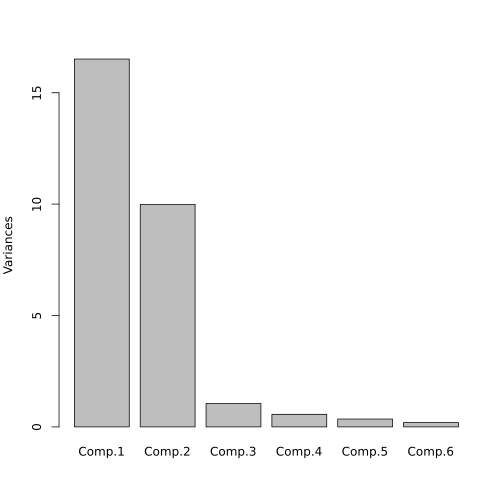
\includegraphics[width=12cm]{images/scree.pdf}
    \caption[Variância capturada pelos PCs]{Variância dos
        dados capturada por cada componente em relação ao
        resultado apresentado na Tabela~\ref{tab:at-pcs}.
        Nota-se que os dois primeiros componentes capturam
        grande parte da variância (aproximadamente $92\%$).}
    \label{fig:scree}
\end{figure}

Muitas perguntas podem surgir a usuários que pretendem
aplicar PCA como simplesmente uma "caixa-preta"~e que são
pouco familiarizados com o processamento interno: o que
significam os componentes, como definir $k$, como definir a
importância de cada componente e assim por diante. Essas
questões poderiam ser evitadas se o usuário fosse incluído
no processo de redução. A Seção~\ref{ss:int} apresenta, um
levantamento de trabalhos que abordam justamente esta
inclusão.

\subsubsection{Seleção de Características} 

O objetivo dos métodos de seleção de características é
encontrar o subconjunto  dos atributos de entrada mais
adequado para a aplicação em estudo. Assim, busca-se
identificar e eliminar atributos
redundantes~\cite{Kohavi1997} ou que não apresentem
correlação com o fenómeno investigado~\cite{Nilsson2007}.
Por exemplo, em tarefas de classificação supervisionada,
pode-se determinar a importância de um atributo avaliando
sua correlação com o atributo classe. Os métodos de seleção
dividem-se basicamente em filtros, \emph{wrappers} e métodos
incorporados~\cite{Guyon2003}. 

Filtros utilizam um atributo alvo como referência e
determinam, por meio de alguma medida de correlação, quanto
cada atributo se relaciona com esta referência. A filtragem
é realizada descartando os atributos que apresentam relação
menor do que um valor fixado. Uma das desvantagens de
filtros é que pelo fato de considerarem somente relações
par-a-par, não são capazes de detectar dependências
indiretas entre os atributos. 

O funcionamento de \emph{wrappers} e métodos embutidos
consiste em realizar uma busca sobre subconjuntos candidatos
e tomar como resultado o subconjunto que resulta na melhor
precisão de um algoritmo de predição. O caso completo
trata-se da avaliação de $2^m$ subconjuntos, onde $m$
corresponde ao número de atributos do conjunto de entrada.
Tal situação equivale a um problema
$np$-completo~\cite{Amaldi1998}, consequentemente para
grandes conjuntos de dados a solução ótima não pode ser
obtida em tempo fazível, exigindo assim a adoção de alguma
eurística. A distinção entre os dois métodos vem de que
\emph{wrappers} enxergam o método de predição como uma
caixa-preta, se interessando somente pelo resultado obtido,
permitindo que diferentes preditores sejam aplicados sem a
necessidade de modificar o método de seleção. Já os métodos
embutidos, como o nome sugere, são incorporados às etapas de
treinamento dos preditores, sendo assim específicos para
cada situação. 

Em comparação aos métodos de extração, os métodos de seleção
apresentam a vantagem de que o resultado obtido é mais
intuitivo ao usuário, pois se trata de um subconjunto dos
atributos de entrada. Assim, se o usuário tem certo
conhecimento sobre o conjunto de entrada, então será capaz
de compreender os resultados obtidos. No entanto, eles
compartilham a mesma natureza caixa-preta dos métodos de
extração e privam o usuário de qualquer interação durante o
processo de redução, impedindo que o usuário contribua com
seu conhecimento sobre o domínio e compreenda quais
características dos seus dados foram responsáveis por aquele
resultado.

\subsection{Métodos Interativos}\label{ss:int}

Métodos visuais que permitem a interação do usuário ganharam
grande popularidade nos últimos anos~\cite{State2012}.
Grande parte deste sucesso pode ser atribuído ao uso efetivo
da capacidade preemptiva da visão humana. Foi demonstrado
que quando os dados são representados por alguma forma
gráfica, o ser humano é capaz de detectar e reconhecer
padrões facilmente e rapidamente~\cite{Healey1995}, mesmo em
grandes conjuntos de dados~\cite{Fodor2002}. Mas a
capacidade preemptiva de visão humana não é a única vantagem
dos métodos visuais. Permitir que o usuário participe
ativamente nos processos e na geração dos resultados é um
dos grandes benefícios desses métodos. Deste
modo, a seguir serão apresentados os trabalhos desta nova
vertente que buscam executar redução de dimensionalidade de
forma interativa. Trabalhos que não somente fazem uso da
capacidade perceptiva dos usuários, mas que também permitem
que o usuário participe ativamente na geração dos resultados
com o seu conhecimento sobre o domínio.

\subsubsection{Matrizes de Correlação}\label{sss:cormat}

\begin{figure}[h!]
    \centering
    \includegraphics[width=10cm]{images/bs1.pdf}
    \caption[Matrizes de Correlação]{Exemplo de matriz de
    correlação para dados de baseball. A cor azul indica
correlação positiva entre as variáveis, enquanto a vermelha
correlação negativa. A intensidade da cor é proporcional à
magnitude da correlação. Com base em uma investigação visual
é possível levantar certas hipóteses sobre os dados.
Observa-se, por exemplo, uma relação direta entre os anos de
carreira do jogador (Years) e o seu salário (logSal), ao
mesmo tempo a experiência tem uma relação inversa com o
número de erros.} 
    \label{fig:bs1}
\end{figure}

Uma das maneiras mais utilizadas para se inspecionar
relações entre dimensões são as matrizes de
correlação~\cite{Friendly2002} (observar
Figura~\ref{fig:bs1}). Este tipo de representação é útil
para se ter uma visão geral das relações entre pares de
dimensões. No entanto, para análises mais detalhadas, ou que
exijam uma comparação entre mais do que simplesmente pares
de elementos, não é uma representação adequada.

\begin{figure}[h!]
    \centering
    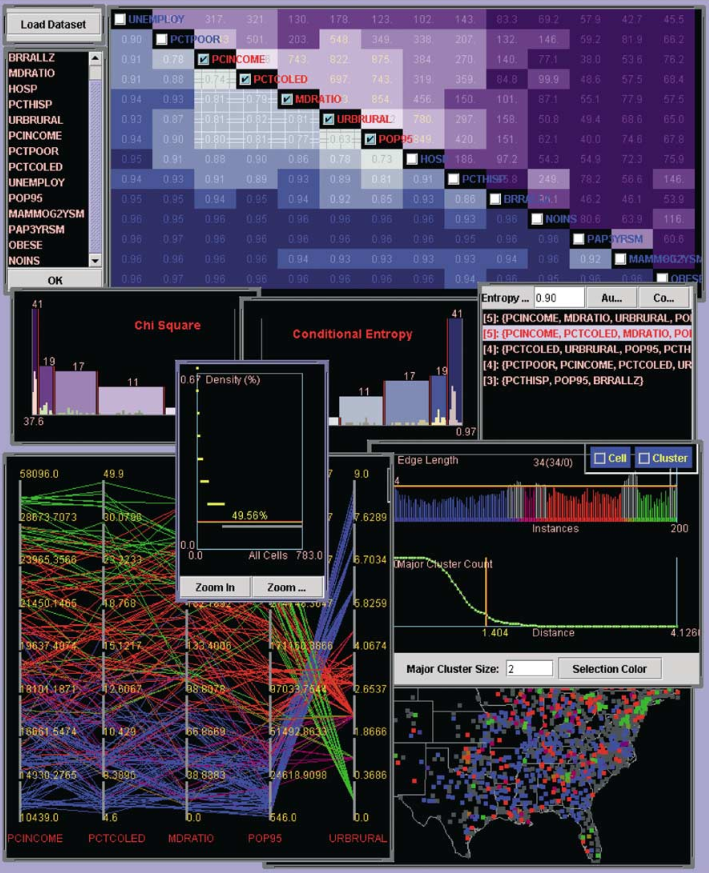
\includegraphics[width=12cm]{images/coord.png}
    \caption[Ferramenta proposta por \cite{Guo2003}]
    {Visão geral do \emph{framework} desenvolvido por
    \cite{Guo2003}. Na parte superior encontra-se a matriz
de correlação. Nota-se que graças ao método de ordenação das
colunas, os grupos de dimensões similares são mais
facilmente identificados. O usuário então seleciona um
subconjunto de atributos por meio da seleção dos elementos
correspondentes na diagonal da matriz. As outras
visualizações são coordenadas com a seleção do usuário e
então análises mais detalhadas podem ser realizadas para uma
melhor compreensão das estruturas presentes naquele
subconjunto de atributos.} 
    \label{fig:coord}
\end{figure}

Devido à sua simplicidade, este tipo de representação foi
adotada por diversos métodos visuais que viabilizam a
investigação de atributos de um conjuntos de dados. O
\emph{framework}\footnote{No contexto deste documento, um
\emph{framework} trata-se de um conjunto de técnicas que são
incorporadas em um ambiente interativo.} desenvolvido por
\cite{Guo2003}, por exemplo, utiliza matrizes de correlação
para apresentar as relações entre os atributos e utilizam um
método de agrupamento para ordenar as colunas da matriz de
modo a destacar grupos de dimensões.

O objetivo da matriz de correlação não é propriamente
reduzir a dimensionalidade do conjunto de dados, mas sim
encontrar subconjuntos de atributos com características
similares. Como é ilustrado na Figura~\ref{fig:coord}, uma
vez identificados esses subconjuntos, o usuário investiga os
grupos de interesse com outros recursos interativos. 

Outros trabalhos
\cite{Friendly2002,MacEachren2003,RBF2004,May2011ss,Johansson2009,Ingram2010,May2011}
também adotam matrizes de correlação para atingir esse mesmo
objetivo. Eles diferem na maneira de como é construída a
matriz de correlação e de quais recursos são
disponibilizados para o usuário interagir com os
subconjuntos de dimensões. Um problema geral desses
trabalhos é que certas análises podem exigir demasiado
esforço do usuário, devido à necessidade de se explorar
individualmente cada dimensão ou avaliar par a par as
relações entre atributos. Com a ocorrência de dependências
não lineares este problema torna-se ainda maior e o usuário
pode se perder em suas análises e não extrair novos
conhecimentos dos resultados. 

\subsubsection{Hierarquias de Dimensões}

Em busca de construir espaços de baixa dimensionalidade mais
intuitivamente do que pelo uso de métodos automáticos,
\cite{Yang2003} desenvolveram o método de redução de
dimensionalidade chamado VHDR (Visual Hierarchical
Dimensions Reduction). O funcionamento deste método é
ilustrado pela Figura~\ref{fig:vhdr1}. Inicialmente
constrói-se uma organização hierárquica dos atributos com
base na similaridade entre as dimensões. Em seguida, com
base nesta hierarquia, o usuário define grupos de dimensões.
Finalmente, o usuário por meio de um método automático ou de
seu conhecimento sobre os dados, escolhe dimensões
representativas para cada grupo, reduzindo assim a
dimensionalidade dos dados. 

\begin{figure}[h!]
  \centering
  \begin{subfigure}[b]{0.35\textwidth}
    \centering
    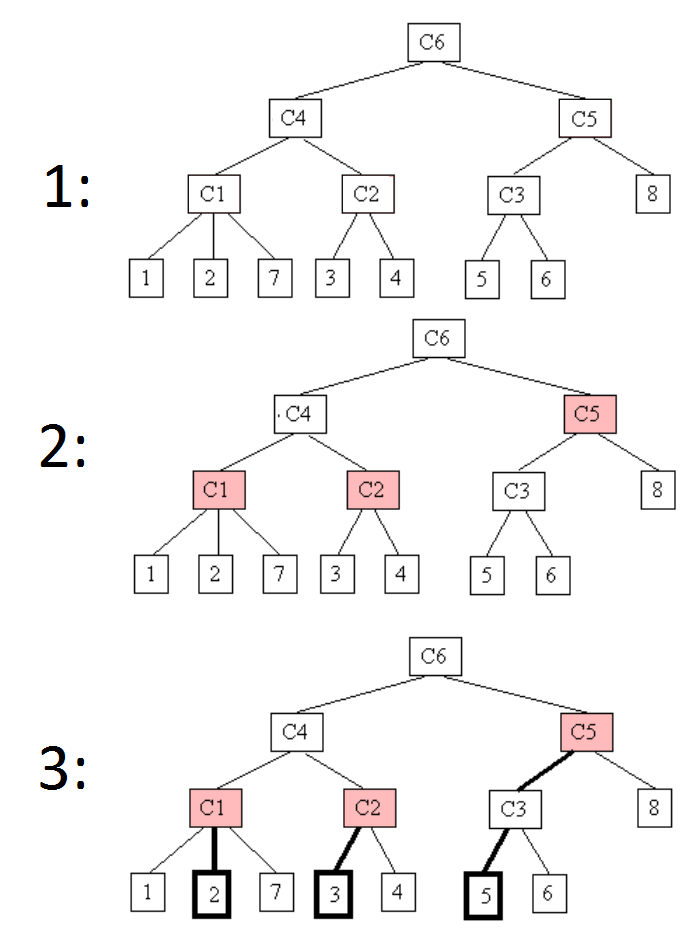
\includegraphics[width=\textwidth]{images/vhdr1.png}
    \caption{}
    \label{fig:vhdr1}
  \end{subfigure}%
  \hspace{1cm} %add desired spacing between images, e. g. ~, \quad, \qquad etc.
  \begin{subfigure}[b]{0.5\textwidth}
    \centering
    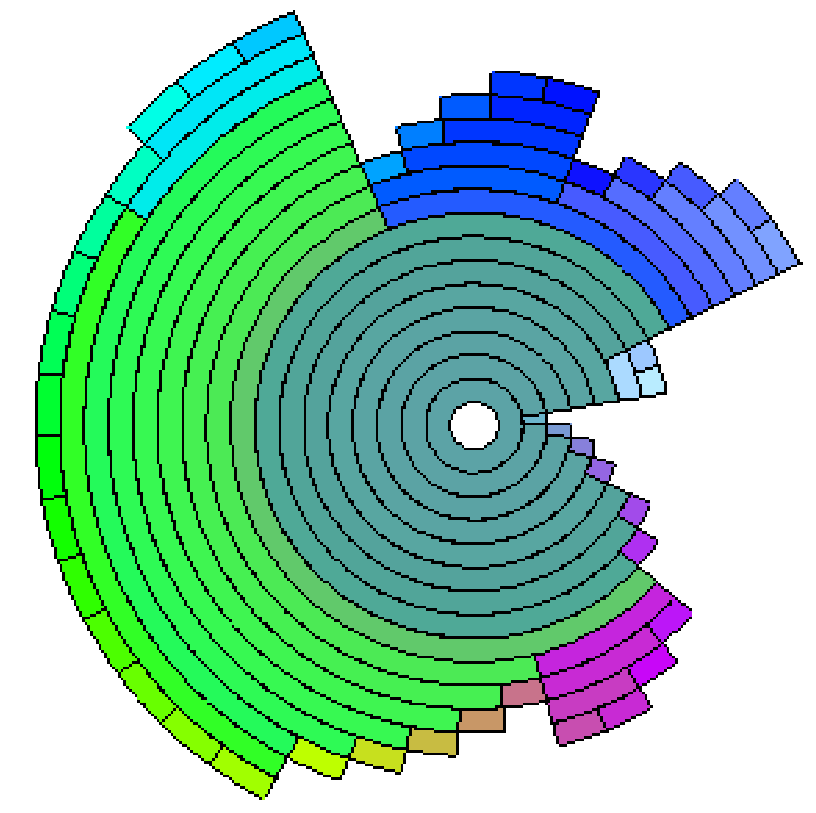
\includegraphics[width=\textwidth]{images/vhdr2.png}
    \caption{}
    \label{fig:vhdr2}
  \end{subfigure}
  \caption[VHDR: Visual Hierarchical Dimension
  Reduction]{(a) Ilustração do funcionamento do VHDR.
  Inicialmente (1), constrói-se uma organização hierárquica
  dos atributos. Em seguida (2), o usuário define grupos de
  dimensões com base na escolha de níveis de cortes da
  árvore. Finalmente (3), o usuário por meio de um método
  automático ou de seu conhecimento sobre os dados, escolhe
  dimensões representativas para cada grupo, reduzindo assim
  a dimensionalidade dos dados. (b) Exemplo da representação
  gráfica InterRing para um conjunto com 42 dimensões e
  $20.000$ elementos. O nó raiz da árvore é representado
  pelo círculo mais interno e os nós folhas pelos elementos
  posicionados na borda. As cores são utilizadas para
  destacar grupos de dimensões com características em
  comum.}
\end{figure}

O processo de construção da hierarquia é muito semelhante
aos algoritmos de agrupamento hierárquico. A distinção é que
agrupa-se atributos semelhantes, ao invés de itens. Deste
modo, qualquer método de agrupamento pode ser aplicado,
exigindo-se apenas que o agrupamento resulte em uma
estrutura hierárquica, no caso uma árvore, onde cada
dimensão seja representada por um nó folha da árvore. 

Uma limitação do VHDR surge quando se inicia a etapa de
seleção de dimensões representativas. A representação visual
não é capaz de transmitir a magnitude da similaridade entre
os atributos. Isto é, o usuário não é capaz de compreender,
por exemplo, quanto um elemento dentro de um grupo é
diferente de outro elemento pertencente a outro grupo. Essa
limitação dificulta tanto a etapa de seleção de grupos
quanto a de escolha de dimensões representativas.

Os autores do VHDR desenvolveram uma extensão chamada DOSFA
(Dimension Ordering Spacing and Filtering
Approach)~\cite{DOSFA} que apresenta outros mecanismos para
manipular os atributos de um conjunto de dados. Mais
especificamente, eles propõem abordagens para ordenação,
espaçamento e filtragem de atributos. As duas primeiras,
ordenação e espaçamento, não estão diretamente relacionadas
com redução de dimensionalidade. Já a filtragem de atributos
é análoga aos métodos de seleção de características. Este
mecanismo consiste em remover dimensões pouco
representativas ou redundantes, de modo que se certas
dimensões apresentam alta similaridade entre si, então
apenas uma delas é mantida, ou se certas dimensões
apresentam pouca relevância, então são descartadas. A grande
complexidade do processo de filtragem é o modo como se
define a redundância e a importância entre as dimensões. Um
método semelhante para filtragem de atributos irrelevantes
foi proposto por \cite{Artero2006}.

Tanto o VHDR quanto o DOSFA tratam todo o conjunto de dados
de maneira uniforme. No entanto, podem existir subconjuntos
nos dados com diferentes características que devem ser
analisados separadamente~\cite{May2011}. Uma maneira de
contornar este problema seria apresentar os itens
simultaneamente com a representação das dimensões, assim o
usuário poderia detectar grupos não somente nas dimensões
mais também nos itens.

\subsubsection{Mapeamento de Elementos no Plano}

Abordando justamente o problema de se apresentar itens
simultaneamente com as dimensões de um conjunto de dados,
\cite{Yang2004} desenvolveram a técnica VaR (Value and
Relation). A técnica une os conceitos de MDS e glifos para
representar as dependências entre as dimensões de uma base
de dados. 

\begin{figure}[h!]
  \centering
  \begin{subfigure}[b]{0.5\textwidth}
    \centering
    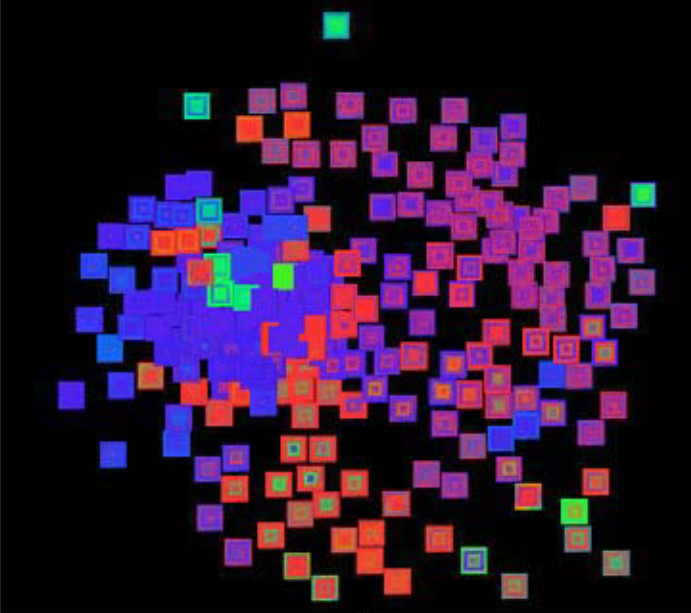
\includegraphics[width=\textwidth]{images/var1.png}
    \caption{}
    \label{fig:var1}
  \end{subfigure}%
  ~ %add desired spacing between images, e. g. ~, \quad, \qquad etc.
  \begin{subfigure}[b]{0.475\textwidth}
    \centering
    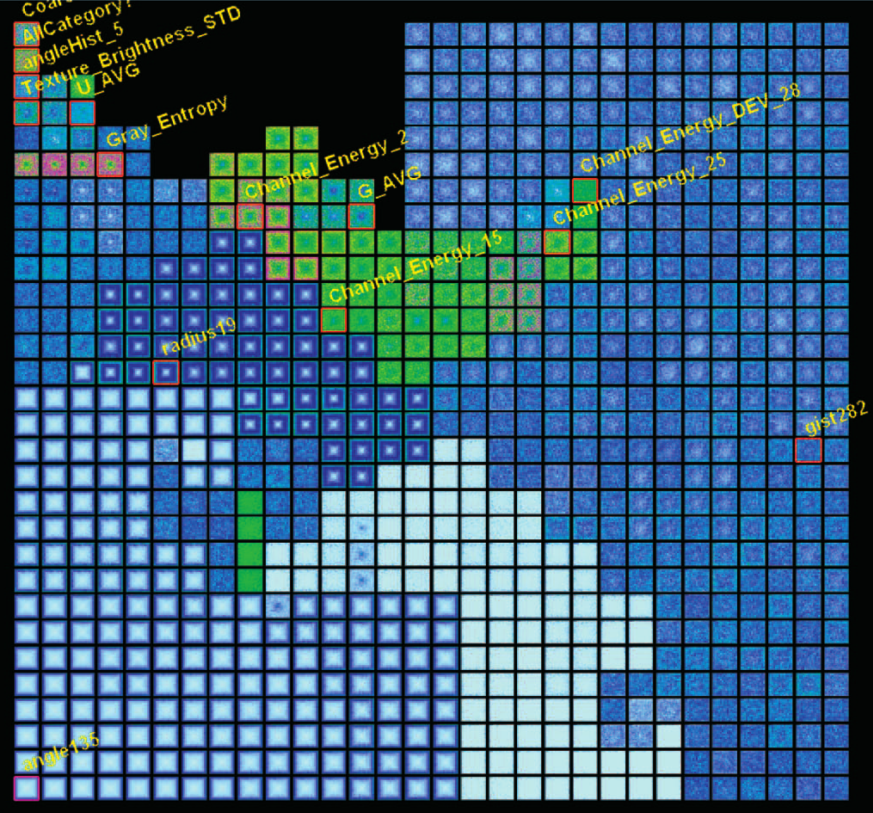
\includegraphics[width=\textwidth]{images/var2.png}
    \caption{}
    \label{fig:var2}
  \end{subfigure}
  \caption[VaR: Value and Relation]{(a) Exemplo da técnica
  VaR para um conjunto de $50.000$ itens e $361$ dimensões.
  Cada dimensão é representada por um glifo e seus
  posicionamentos refletem a similaridade entre as
  dimensões, de modo que glifos que se encontram próximos
  indicam atributos que apresentam alguma relação entre si.
  É possível notar certas sobreposições entre os glifos,
  condição que pode dificultar as análises realizadas pelo
  usuário. (b) Exemplo de representação alternativa proposta
  como extensão da técnica VaR para um conjunto de 11.413
  itens e 838 dimensões. O principal objetivo desta
  representação alternativa é evitar sobreposições de glifos
  ocorrente na versão anterior da técnica.}
\end{figure}

Como mostra a Figura~\ref{fig:var1}, cada glifo representa
uma dimensão e de acordo com seus posicionamentos no plano o
usuário pode compreender como as dimensões se relacionam
entre si.  O usuário é capaz de construir espaços
dimensionais reduzidos que conservam certas características
dos dados por meio de seleções sobre os dados ou pelo uso de
um método automático que a partir de uma dimensão de
referência e um limiar definido pelo usuário retorna as
dimensões mais semelhantes.

O procedimento para a construção desta visualização inicia
pela construção de uma matriz de distâncias que é
responsável por capturar os relacionamentos entre pares de
dimensões do conjunto de dados.  Sobre esta matriz de
distâncias aplica-se uma técnica de MDS para mapear cada
dimensão em uma posição do espaço bidimensional.
Finalmente, cria-se um glifo orientado a pixels para cada
dimensão que será utilizado para representar cada dimensão
no plano.

Observando a Figura~\ref{fig:var1} é possível notar que o
uso de glifos faz com que ocorram sobreposições, pois cada
glifo requer um espaço relativamente grande para que seja
observado adequadamente.  As sobreposições dificultam as
análises de regiões de interesse e podem fazer com que o
usuário alcance conclusões inválidas, devido a oclusão de
algum elemento importante.  Buscando tratar este
problema~\citeauthor{Yang2007} desenvolveram a
extensão~\cite{Yang2007} ilustrada na Figura~\ref{fig:var2}
para a técnica VaR, onde apresentaram alternativas para a
projeção de glifos no plano. No entanto, por estabelecerem
uma distância fixa entre os elementos, perde-se a informação
de quanto duas dimensões são similares entre si. Assim, a
alternativa proposta não é capaz de transmitir os
relacionamentos entre as dimensões tão bem quanto o
resultado obtido pela versão original.

Apesar do método VaR apresentar informações sobre itens e
dimensões simultaneamente, não é permitido ao usuário
interagir com os itens. Consequentemente, este método sofre
das mesmas limitações dos métodos apresentados
anteriormente, ou seja, não é capaz de tratar peculiaridades
em subconjuntos dos dados.  Um outro aspecto importante que
os próprios autores mencionam em relação ao uso deste tipo
de glifos é que os usuários têm dificuldade em comparar
glifos que se encontram afastados entre si. 

\begin{figure}[h!]
  \centering
  \begin{subfigure}[b]{0.45\textwidth}
    \centering
    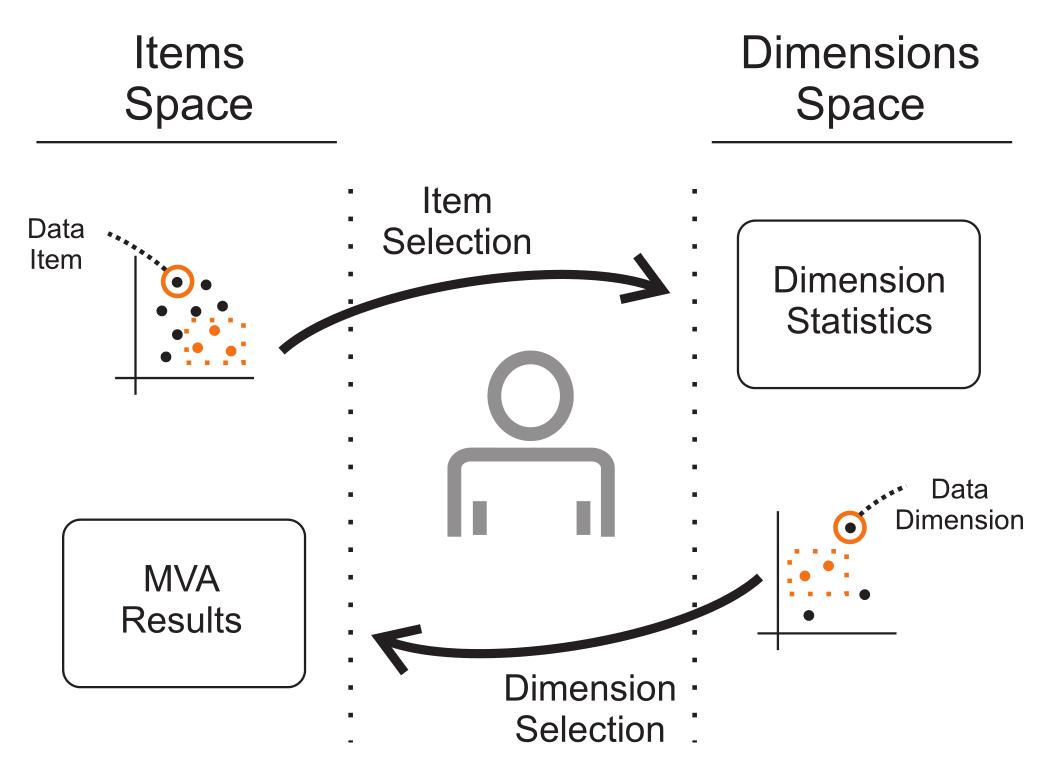
\includegraphics[width=\textwidth]{images/bd1.png}
    \caption{}
    \label{fig:bd1}
  \end{subfigure}%
  \begin{subfigure}[b]{0.55\textwidth}
    \centering
    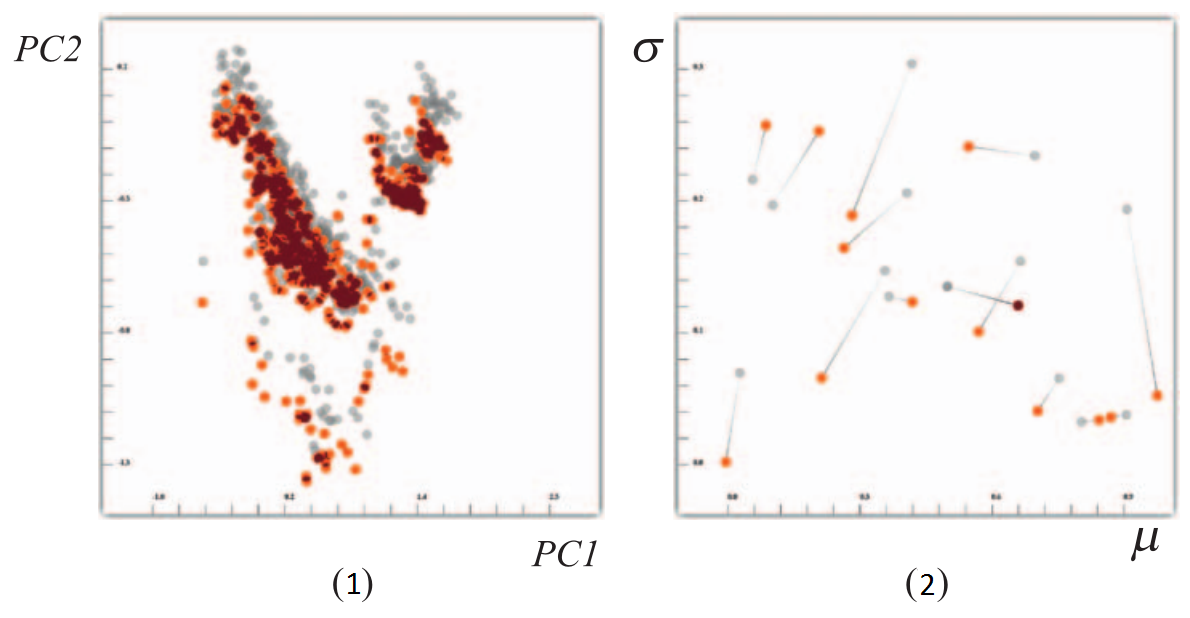
\includegraphics[width=\textwidth]{images/bd2.png}
    \caption{}
    \label{fig:bd2}
  \end{subfigure}
  \caption[Brushing Dimensions]{Ilustração do método
  Brushing Dimensions. Em (a) apresenta-se o conceito de
  interação tanto com itens quanto com dimensões. As
  representações dos itens são construídas com base em
  métodos automáticos, como PCA, e as das dimensões por
  medidas estatísticas, como média e variância. O usuário
  pode realizar seleções em ambas as representações, em (b)
  apresenta-se uma seleção nos itens em (1) e as alterações
  nas posições das dimensões em (2).}
  \label{fig:bd}
\end{figure}

Semelhantemente ao método VaR, o trabalho proposto por
\cite{Turkay2011}, \emph{Brushing Dimensions} (BD) apresenta
representações visuais de itens e dimensões simultaneamente
por meio do mapeamento de elementos no plano
(Figura~\ref{fig:bd}). O método também mapeia as dimensões
no plano, mas não faz uso de métodos de MDS  para isso.
Utiliza uma abordagem mais simples, onde à cada dimensão é
atribuída uma posição no plano de acordo com sua média e
variância. Este modo de posicionamento é uma das limitações
do método, pois ao desconsiderar medidas par-a-par, como
correlação, o usuário não consegue identificar dependências
entre os atributos.

Uma vantagem do BD sobre o VaR é a possibilidade do usuário
interagir tanto com itens quanto com dimensões. O principal
mecanismo de interação deste método é a seleção que se
reflete em outras visões e permite que se visualize, por
exemplo, variações na importância de um atributo em
diferentes subconjuntos dos dados. Uma das limitações de
ambos os métodos, VaR e BD, trata-se de não permitir que o
usuário construa novas dimensões com base nas originais ou
com base no seu conhecimento.

Uma questão inerente de se mapear elementos de um espaço de
alta dimensionalidade em um plano, sejam os elementos itens
ou dimensões, é que não há garantias de que o mapeamento
seja válido. Em casos onde a dimensionalidade intrínseca dos
dados for maior do que ao do espaço alvo, então poderá haver
sobreposição de elementos sem necessariamente significar que
os elementos sobrepostos sejam realmente semelhantes. Ambos
VaR e BD não atentam para esta questão, mas
\cite{Ingram2010} desenvolveram a ferramenta
\emph{DimStiller} (DS) buscando construir mapeamentos de
dados multidimensionais levando em consideração este
problema. 

\begin{figure}[h!]
    \centering
    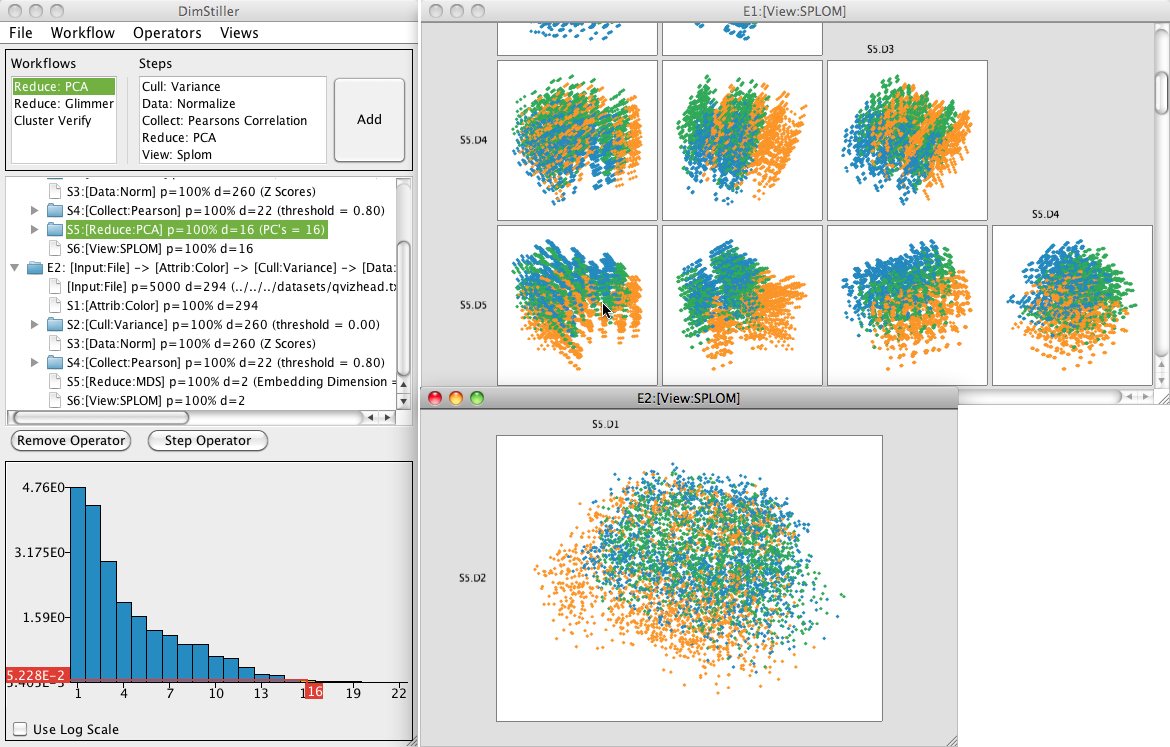
\includegraphics[width=16cm]{images/ds.png}
    \caption[DimStiller]{Abordagem proposta pela ferramenta
    \emph{DimStiller} para criar mapeamentos de dados
multidimensionais interativamente. Pelo gráfico de barras
(janela canto inferior esquerdo) o usuário atenta para a
dimensionalidade intrínseca dos dados e para os limites da
redução de dimensionalidade. O mapeamento resultante da
redução é apresentado em um gráfico dos dois componentes
principais (janela canto inferior direito). De acordo com
esta visualização, não existem estruturas de interesse nos
dados. No entanto, ao observar mapeamentos com outros
componentes da redução (janela canto superior direito), o
usuário pode identificar certos padrões nos dados.}
    \label{fig:ds}
\end{figure}

Um outro aspecto importante da redução de dimensionalidade,
que muitas vezes não é levado em consideração, trata-se que
dependendo do método adotado, diferentes características dos
dados podem ser mantidas e outras perdidas. Este problema é
abordado no trabalho de \cite{Johansson2009}, onde por meio
de gráficos de perda de informação para diferentes medidas o
usuário pode entender quais características dos seus dados
são mantidas e perdidas ao longo do processo de redução.
Este trabalho, assim como o \emph{DimStiller}, permite que o
usuário reduza a dimensionalidade dos conjuntos de dados por
meio da interação sobre matrizes de correlação.
Consequentemente, esses métodos compartilham das limitações
do uso dessas matrizes descritas na
Subseção~\ref{sss:cormat}.

\subsubsection{Visualização de Métodos Automáticos}

\begin{figure}[h!]
    \centering
    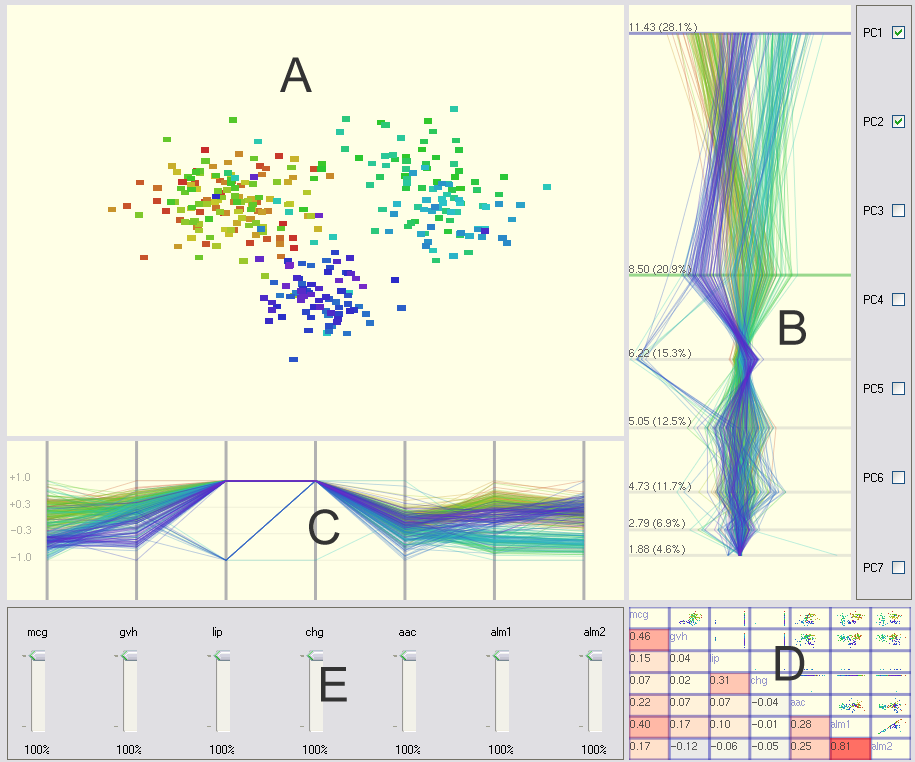
\includegraphics[width=14cm]{images/ipca.png}
    \caption[iPCA]{Ilustração da técnica iPCA. Em (A)
    apresenta-se o mapeamento dos elementos no plano
utilizando dois componentes principais selecionados pelo
usuário. (B) e (C) referem-se a visualizações dos dados
originais e transformados, respectivamente. Em (D) é
apresentada uma matriz de correlação. O principal mecanismo
de interação é indicado por (E), o qual permite ao usuário
definir a contribuição de cada atributo no resultado final.}
    \label{fig:ipca}
\end{figure}

Existem métodos que não fazem uso de representações
visuais para realizar a redução de dimensionalidade em si,
mas sim para tornar os métodos de redução automática mais
compreensivos. Eles buscam incluir a participação do usuário
nesses métodos para tornar essas ``caixas pretas'' mais
intuitivas. 

A técnica iPCA~\cite{Jeong2009}, por exemplo, provém meios
para o usuário manipular os parâmetros da técnica PCA e,
assim, ser capaz de entender mais facilmente as
transformações realizadas sobre os dados. Similarmente,
\cite{Williams2004} permite que o usuário guie o processo de
redução de dimensionalidade a partir de métodos MDS ao
escolher regiões de interesse para se concentrar os esforços
computacionais.

Dentro do contexto de seleção de características, o trabalho
de \cite{Dy2000} busca tornar este processo mais interativo.
Possibilitando ao usuário escolher grupos de itens para
análises mais detalhadas e fornecendo mecanismos interativos
para adição e remoção de atributos em cada etapa dos métodos
de seleção. O trabalho de \cite{Brandoli2010} apresenta um
objetivo similar, porém com um enfoque em auxiliar o
usuário a definir os parâmetros dos métodos de seleção de
características.

Os trabalhos propostos por \cite{Choo2010}, \cite{Paiva2012}
e \cite{Zhang2006} são abordagens que buscam não somente
tornar o processo de redução de dimensionalidade mais
intuitivo, mas que também são aplicáveis no contexto de
classificação de dados. Nesses métodos a redução de
dimensionalidade reflete diretamente a qualidade das
classificações. 

Um problema dos métodos que criam visualizações de métodos
automáticos é a necessidade do usuário ter um certo
conhecimento do método por trás da visualização. Por
exemplo, no caso da ferramenta iPCA, o usuário pode ver
pouca utilidade na visualização da janela se não souber o
que significa um componente principal. Para pesquisadores da
área pode ser até pressuposto que o usuário tenha este tipo
de conhecimento, no entanto, se o objetivo for
criar uma ferramenta para o público em geral, então tal
suposição pode restringir o seu uso.

\section{Transformação Interativa do Espaço de Atributos}

Os métodos de redução de dimensionalidade realizam
transformações sobre os dados, porém, mesmo os métodos
interativos de redução não permitem que o usuário modifique
os atributos livremente. Os métodos de transformação
interativa do espaço de atributos buscam mais do que somente
permitir que o usuário guie as transformações sobre os
dados, eles permitem que o usuário modifique os atributos
diretamente. Tais métodos não contam com uma literatura tão
vasta quanto a dos métodos de redução de dimensionalidade,
mas têm ganhado popularidade nos últimos anos,
particularmente em aplicações de avaliação de funções
multidimensionais~\cite{Jayaraman2002,Weber2007,Matkovic2008,
Guo2009}. 

No contexto de aplicações industriais, \cite{Berger2011}
desenvolveram um método para investigação de como os
parâmetros de uma função afetam o seu resultado e também
como os parâmetros podem ser modificados para se atingir um
valor desejado. No entanto, como mostra a
Figura~\ref{fig:berger}, os mecanismos de interação
propostos se baseiam em interfaces que são
demasiadamente complexas o que dificulta as análises,
principalmente quando o usuário lida com um grande volume de
dados.

\begin{figure}[h!]
    \centering
    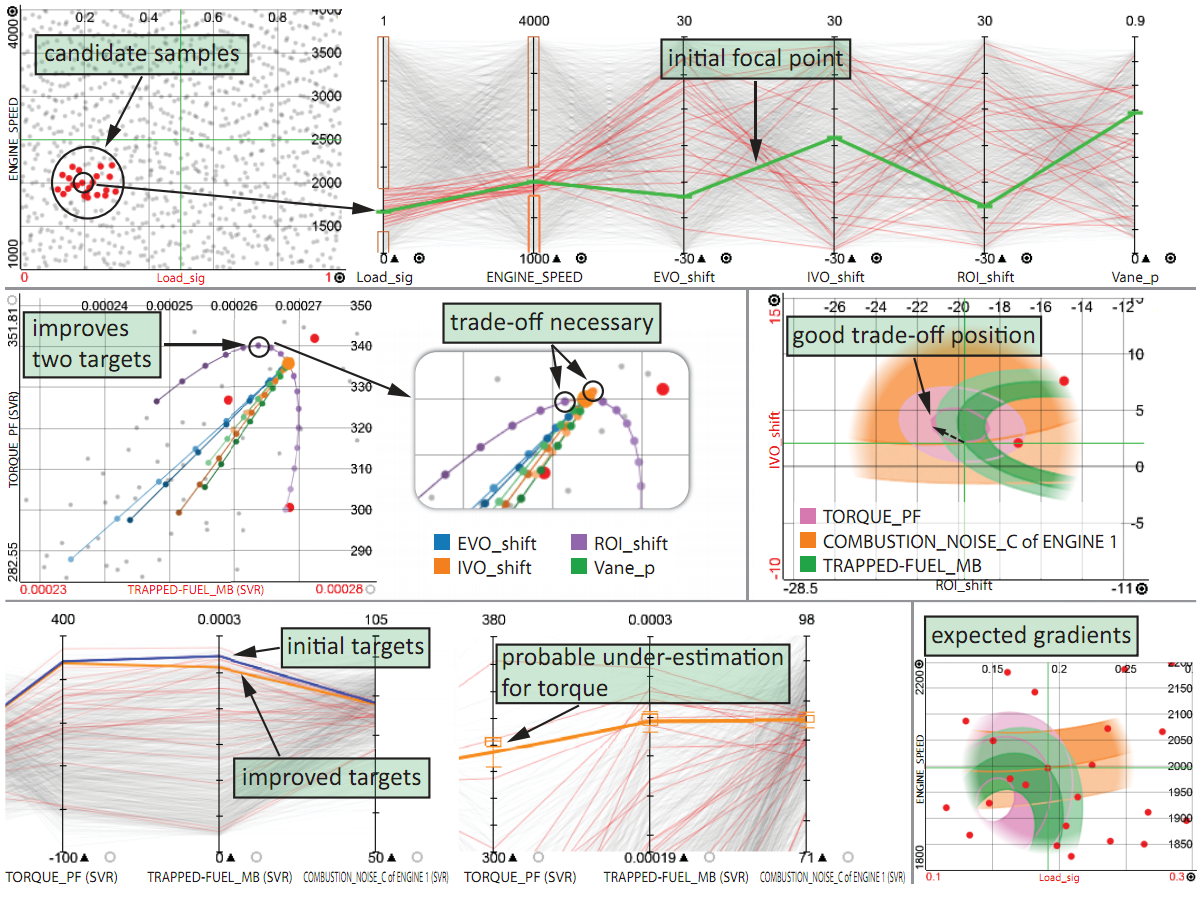
\includegraphics[width=16cm]{images/berger.png}
    \caption[Ferramenta proposta por \cite{Berger2011}]
    {Ferramenta proposta por \cite{Berger2011}. Mais do que detalhar cada janela, pretende-se ilustrar com
esta figura a complexidade da ferramenta. O usuário interage
com uma variedade de representações visuais, onde cada uma exige
um modo particular de análise.}
    \label{fig:berger}
\end{figure}

Mais recentemente, \cite{Gladys2013} desenvolveram o
\emph{framework User-driven Feature Space Transformation}
(UDFST) que possibilita ao usuário modificar os
atributos de um conjunto de dados com base na manipulação
sobre amostras dos itens. Neste trabalho os autores se
preocuparam em não sobrecarregar o usuário com interfaces  
demasiadamente complexas. Eles fazem uso de mapeamento de
elementos no plano para permitir interações mais intuitivas.


Como mostra a Figura~\ref{fig:ud}, o método UD-FST parte de uma
amostragem dos dados, a qual o usuário manipula
para agrupar elementos que considera similares. Em seguida,
as manipulações realizadas sobre a amostra são refletidas
para o conjunto de dados original, fazendo com que este
reflita a opinião do usuário em relação ao critério de
similaridade entre os elementos.

\begin{figure}[h!]
    \centering
    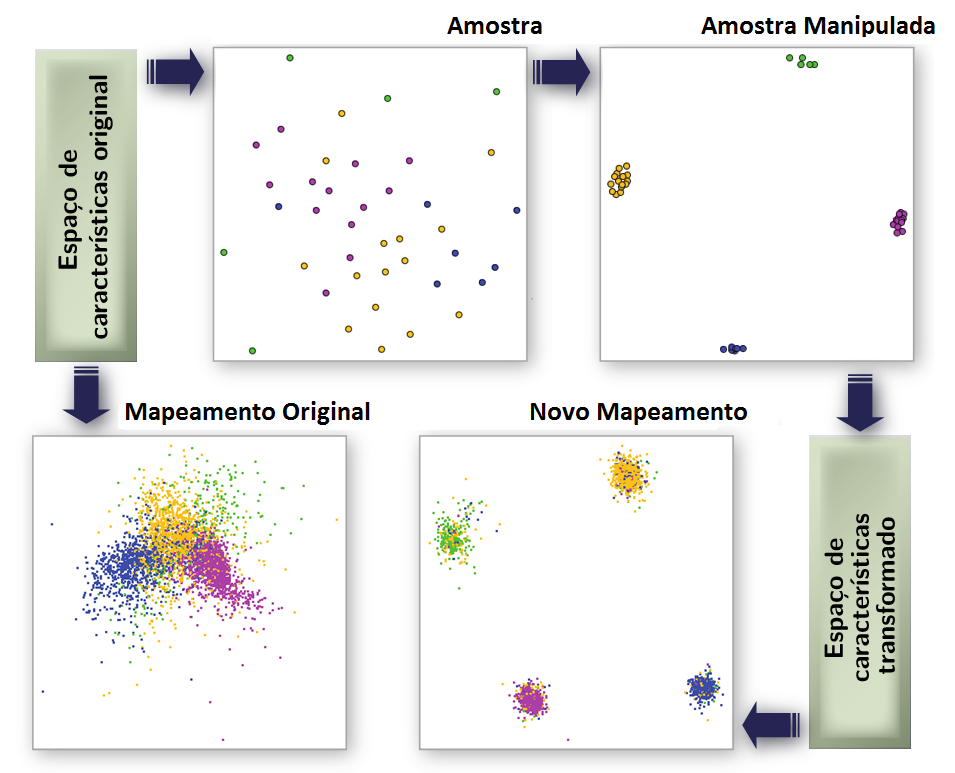
\includegraphics[width=16cm]{images/ud.png}
    \caption[Ferramenta desenvolvida por \cite{Gladys2013}]
    {Ferramenta desenvolvida por \cite{Gladys2013}. O método
    parte de uma amostragem dos dados, a qual o usuário
    manipula para agrupar elementos que considera
    similares. Em seguida, as manipulações realizadas
    sobre a amostra são refletidas para o conjunto de
    dados original, fazendo com que este reflita a
    opinião do usuário em relação ao critério de
    similaridade entre os elementos. Este processo pode
    ser repetido iterativamente até que se atinja o
    resultado esperado. Observa-se que para este
    exemplo a transformação do espaço foi bem sucedida, pois
    foram reveladas estruturas que até então não eram
    identificáveis.}
    \label{fig:ud}
\end{figure}

Certos fatores afetam drasticamente o resultado obtido
pelo UD-FST. Trata-se do caso da maneira que se
escolhe a amostra dos dados. Utilizando, por exemplo, uma
amostragem aleatória, não haveriam garantias de que
elementos de cada estrutura seriam escolhidos.
Consequentemente, o usuário precisaria de mais iterações
para agregar aos dados o seu conhecimento.

\section{Considerações Finais}

Neste capítulo foram apresentados os trabalhos que modificam
os conjuntos de dados de modo a torná-los mais
representativos para a compreensão do fenómeno em estudo.
Métodos visuais que permitem a interação do usuário
receberam uma atenção especial. No entanto, como é
apresentado na Tabela~\ref{tab:tr}, individualmente esses
métodos não possuem todos os mecanismos necessários para a
transformar os dados efetivamente.

\newcommand{\redc}{\cellcolor{red!25}Não}
\newcommand{\greenc}{\cellcolor{green!25}Sim}

\begin{table}
    \centering
    \caption[Mecanismos interativos dos trabalhos relacionados.]
    {Principais mecanismos de interação dos trabalhos
    relacionados. Observa-se que nenhum dos métodos
    consegue unir os três um único ambiente.}
    \begin{tabular}{|C{4cm}|C{3cm}|C{3cm}|C{3cm}|}
        \hline
        \textbf{Técnica} &
        \textbf{Seleção} &
        \textbf{Extração} &
        \textbf{Transformação} \\
        \hline
        Matrizes de Correlação  & \greenc & \redc & \redc \\    
        \hline
        VHDR                    & \greenc & \redc & \redc \\ 
        \hline
        DOSFA                   & \greenc & \redc & \redc \\ 
        \hline
        Value and Relation      & \greenc & \redc & \redc \\ 
        \hline
        Brushing Dimensions     & \greenc & \redc & \redc \\ 
        \hline
        DimStiller              & \greenc & \greenc & \redc \\ 
        \hline
        iPCA                    & \redc & \greenc & \redc \\ 
        \hline
        UD-FST                  & \redc & \redc & \greenc\\ 
        \hline
    \end{tabular}
    \label{tab:tr}
\end{table}
